% die Standard-Dokumentenklasse
\documentclass[11pt,a4paper]{article} %% 1.Ebene = chapter, headings

% input encoding, font encoding, outline font
\usepackage[utf8]{inputenc} 
\usepackage[T1]{fontenc} 
\usepackage{lmodern}
\usepackage{tcolorbox}
% Sprache
\usepackage[german]{babel}

% Absatzformatierung
\setlength{\parindent}{0pt}
\setlength{\parskip}{1ex plus 0.5ex minus 0.5ex}

% erweiterte mathematische Symbole
\usepackage{amsmath} 

% für Abbildungen
\usepackage{graphicx} 

% für Tabellen
\usepackage{booktabs}

% für Hyperlinks
\usepackage[colorlinks]{hyperref}
\graphicspath{}

%%%%%%%%%%%%%%%%%%%%%%%%%%%%%%%%%%%%%%%%%
\begin{document}
	
	
	{
		\centering 
		\large 
		Physiklabor für Anfänger*innen \\
		Ferienpraktikum im Sommersemester 2018 \\[4mm]
		\textbf{\LARGE 
			Versuch 38: Spezifische Wärmekapazität von Wasser
		} \\[3mm]
		(durchgeführt am 10.09.2018 bei Nico Strauß) \\
		Ye Joon Kim, Marouan Zouari\\
		\today \\[10mm]
	}
\section{Einleitung}
Die Erhaltung der Energie impliziert, dass die Energie in andere Formen umgewandelt werden können. Insbesondere können mechanische und elektrische Energie sich in thermische Energie umwandeln. Mit dieser Eigenschaft lässt sich die Wärmekapazität von Wasser bestimmt werden. Mit Reibung können mechanische Arbeit in Wärme umgewandelt werden. Mit einem Schürholz-Apparat kann das anschaulich gemacht werden. Das Stromwärmegesetzt besagt, dass die von einem Widerstand abgegebene Wärme proportional zur Spannung und Strom ist. Dadurch lässt sich elektrische Energie in Wärme umwandeln. 

\section{Ziel des Versuchs}
Das Ziel dieses Versuchs ist es, die spezifische Wärmekapazität von Wasser auf mechanische und elektrische Weise zu bestimmen (nämlich mit einem Schurholz-Apparat und einem Widerstand).  
\section{Aufbau}
Abbildungen auf n\"{a}chste Seite .

\begin{figure}
	\centering
	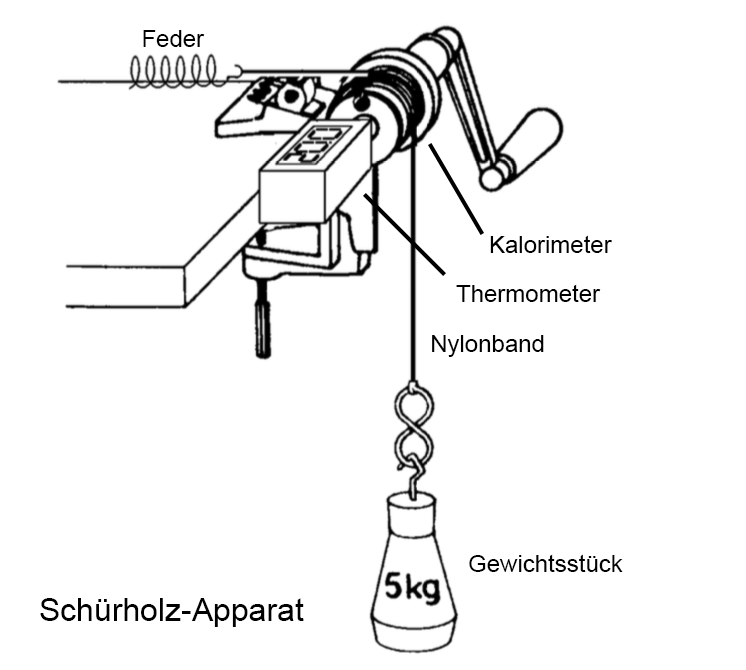
\includegraphics[scale=0.5]{fig1}
	\caption{Schürholz-Apparat: Versuchsaufbau zur Bestimmung der spezifischen Wärmekapazität von
		Wasser auf mechanischem Weg.}
	
	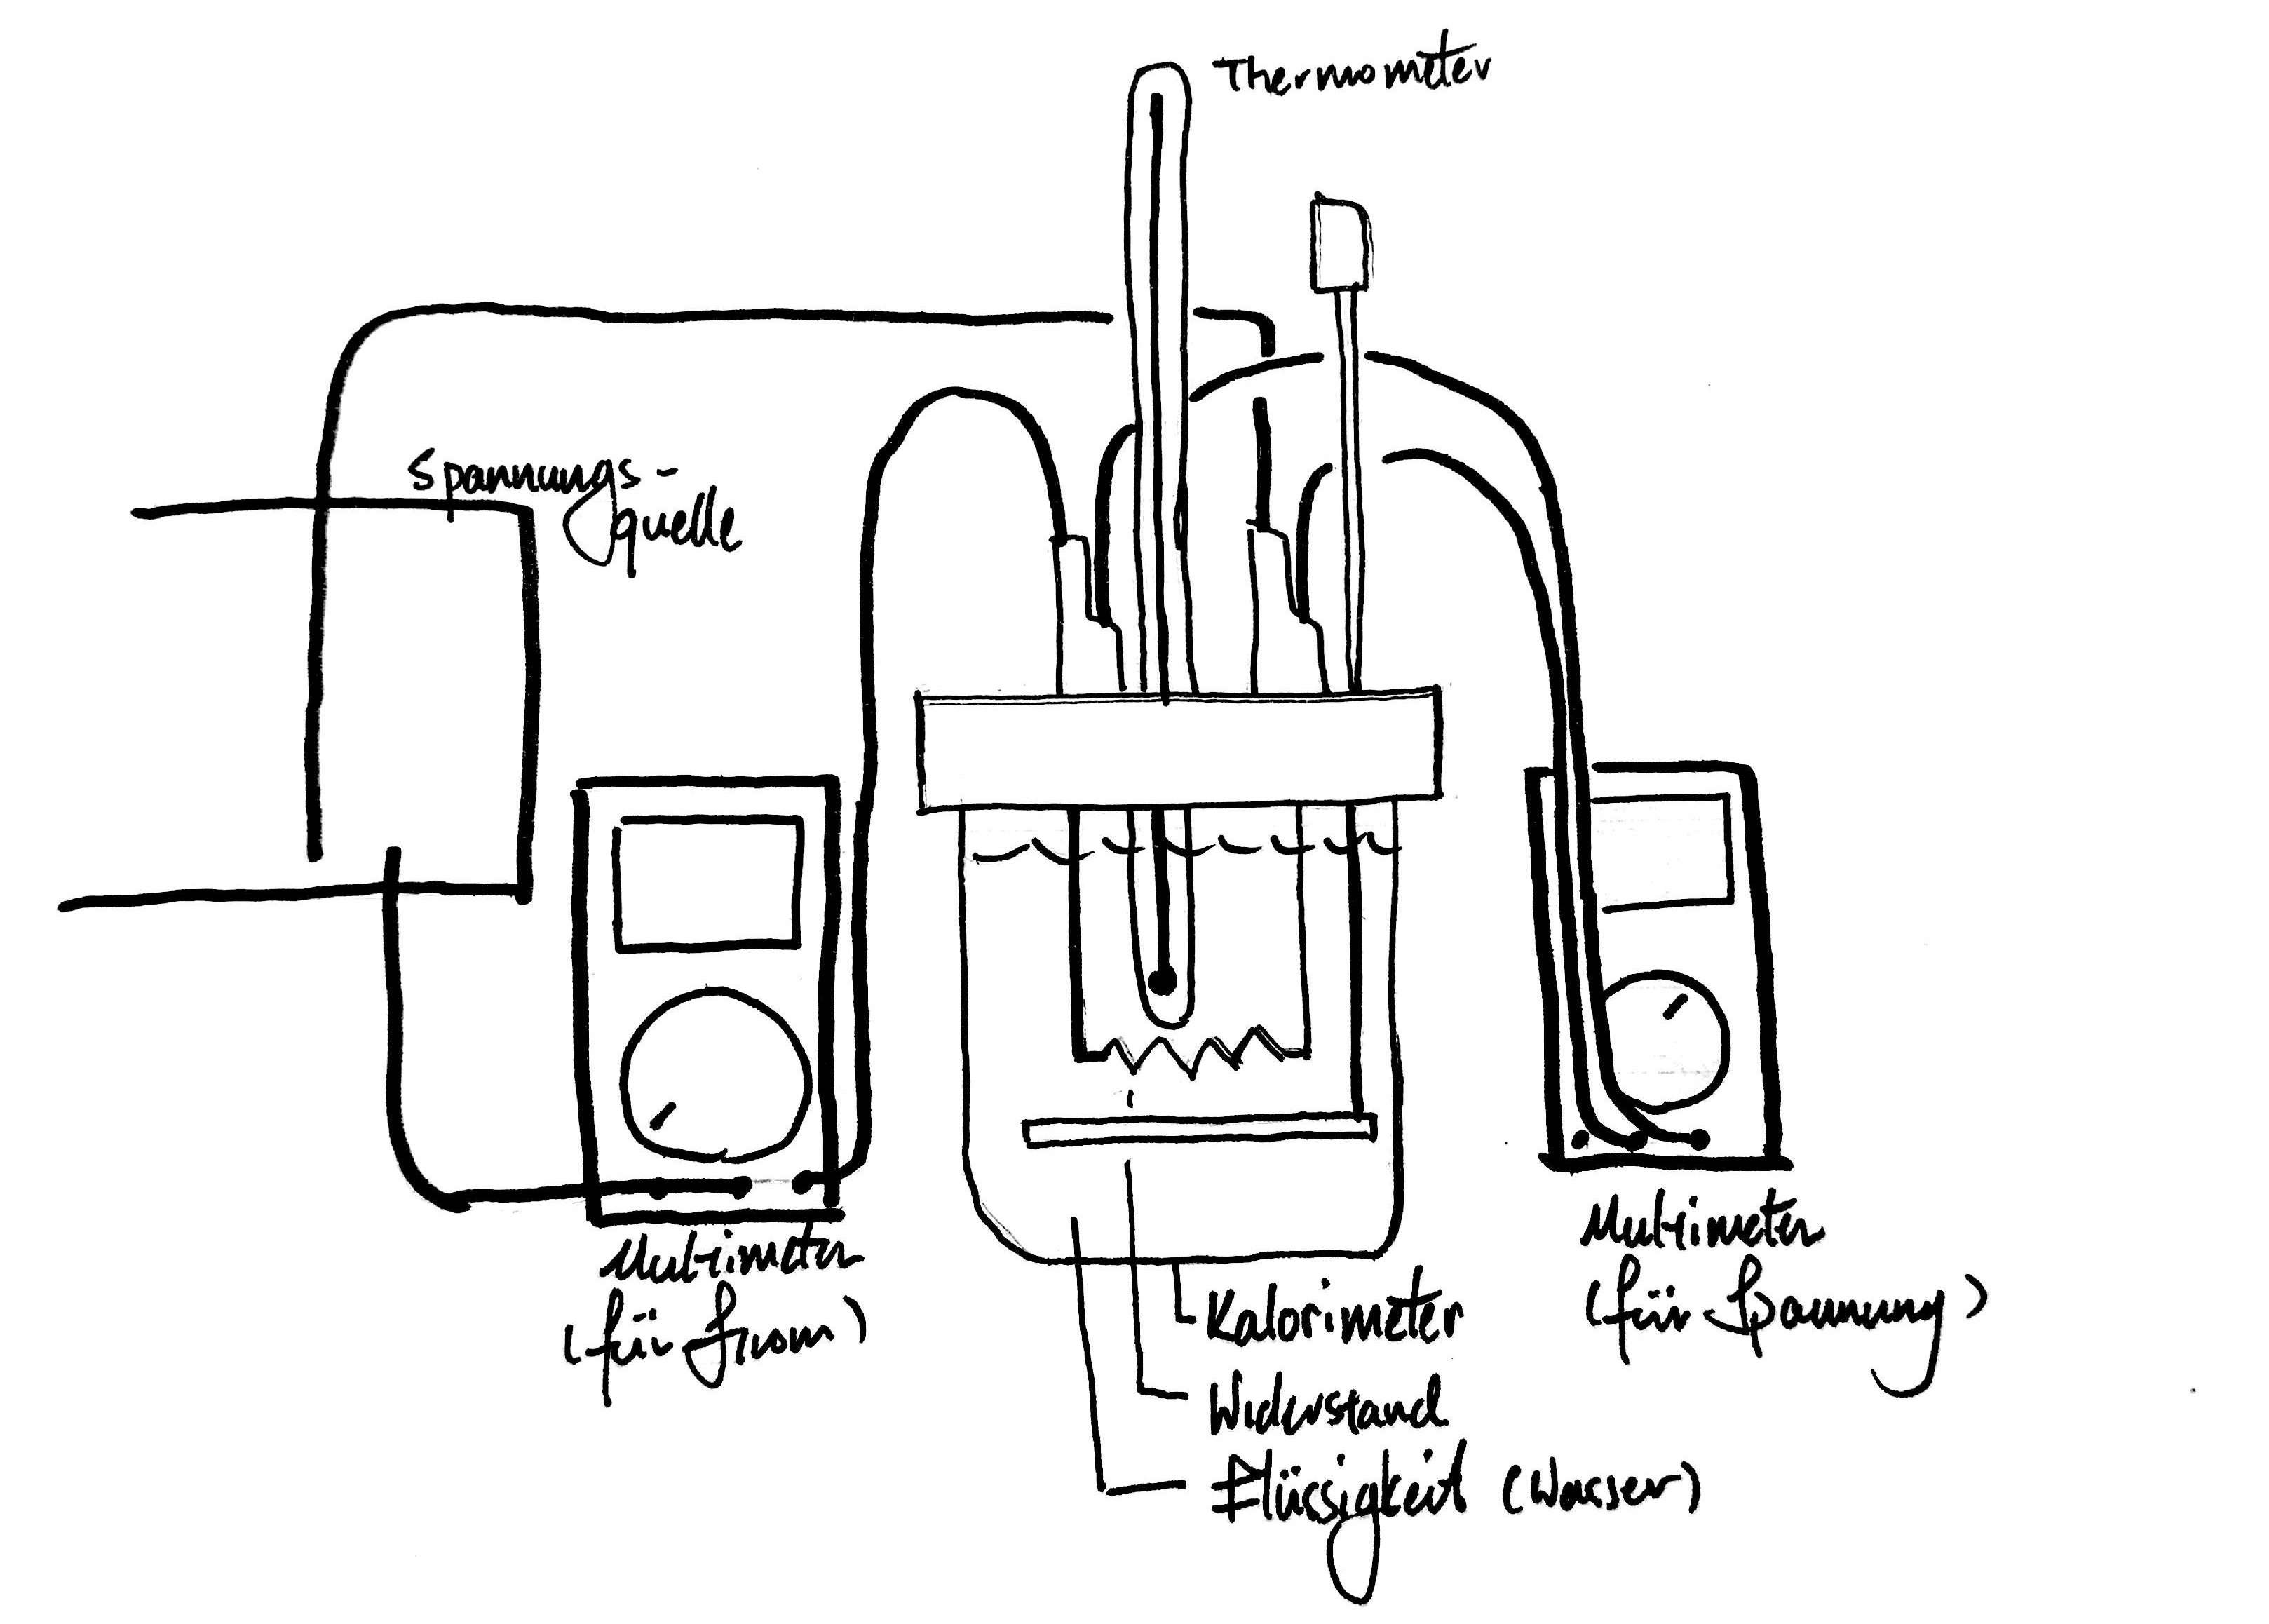
\includegraphics[scale=0.10]{fig2}
	\caption{ Versuchsaufbau zur Bestimmung der spezifischen Wärmekapazität von
		Wasser auf elektrischem Weg.}
\end{figure}
\newpage

\section{Auswertung und Fehlerrechnung}
Rohe Daten sind in dem Anhang zu finden. 

\subsection{1. Versuchsteil:Mechanische Bestimmung der Wärmekapazität.}

Für die Bestimmung der Wärmekapazität wird die folgende Formel benutzt:
\begin{equation}
(\Gamma_{\textrm{Kal}}+\Gamma_{\textrm{T}}+m_\textrm{W}c_\textrm{W})\Delta T = mgn\pi d
\end{equation}
wobei:
\begin{itemize}
	\item $\Gamma_{\textrm{Kal}}$ Die Wärmekapazität des leeren Kalorimeters
	\item $\Gamma_{\textrm{T}}$ Die Wärmekapazität der Thermoelemententhalterung und des Nylonbands
	\item $m_\textrm{W}$ Die Masse des Wassers
	\item $c_\textrm{W}$ Die spezifische Wärmekapazität des Wassers
	\item $\Delta T$ die Temperaturunterschied
	\item $m$ die Masse des Massestücks
	\item $g$ die Fallbeschleunigung
	\item $n$ die Anzahl Drehungen
	\item $d$ der Durchmesser des Kalorimeters sind
\end{itemize}

Die Formel kann umgeformt werden, um einen Ausdruck für $c_\textrm{W}$ zu liefern:

\begin{equation}
c_\textrm{W} = \frac{\frac{mgn\pi d}{\Delta T} - \Gamma_{\textrm{Kal}} - \Gamma_{\textrm{T}}}{m_\textrm{W}}
\end{equation}



Es wurden vier Messungen durchgeführt. Die von den Einzelmessungen gewonnenen Werte für die spezifische Wärmekapazität und deren Unsicherheiten sind:


\begin{table}[h]
	\centering
	\begin{tabular*}{0.99\textwidth}{@{\extracolsep{\fill}}cccccc}
		\toprule
		Messreihe & $c_\textrm{W}$ & $\Delta( c_\textrm{W})$  \\
		& J/kg K & J/kg K   \\
		\bottomrule
		1 & $5,44298 \cdot 10^{3}$ & $2,02625 \cdot 10^{3}$ \\
		2 & $5,8 \cdot 10^{3}$ & $1,1 \cdot 10^{3}$ \\
		3 & $6,2 \cdot 10^{3} $& $1,3 \cdot 10^{3}$ \\
		4 & $6,2 \cdot 10^{3}$ & $1,3 \cdot 10^{3}$ \\
		\bottomrule
	\end{tabular*}
	\caption{Die berechneten Werte für  $c_\textrm{W}$ und deren  Unsicherheiten}
	\label{tabelle}
\end{table}

\begin{tcolorbox}[colback=white]
\textbf{Beispielrechnungen (Mit ersten Datenpunkten)}	

Einfaches Einsetzen der Werte in Gleichung (2) liefert die jeweilige spezifische Wärmekapazitäten. 
$$c_\textrm{W} = \frac{\frac{mgn\pi d}{\Delta T} - \Gamma_{\textrm{Kal}} - \Gamma_{\textrm{T}}}{m_\textrm{W}}$$

$$ =\frac{ \frac{ 5 \textrm{kg} \cdot 9,8 \textrm{m/s}^2 \cdot 50 \cdot \pi \cdot 0,0472 \textrm{m}}{0,9^\circ C} - (380 \textrm{J/kg K} \cdot 0,098 \textrm{kg}) - 5 \textrm{J/K}}{0,066\textrm{kg}}$$
$$ = 5442,98 \textrm{J/kg K} $$
Und für die Fehlerrechnungen werden die Gauß'sche Fehlerfortpflanzung benutzt. Mit:
$$f(n,d,\Delta T,m_\textrm{W}) = \frac{\frac{mgn\pi d}{\Delta T} - \Gamma_{\textrm{Kal}} - \Gamma_{\textrm{T}}}{m_\textrm{W}}$$
sind:
$$ \frac{ \partial f}{\partial n} = \frac{mg\pi d}{\Delta T m_{\textrm{W}}} $$ 
$$ \frac{ \partial f}{\partial d}  = \frac{mgn\pi}{\Delta Tm_{\textrm{W}}}$$
$$ \frac{\partial f}{\partial \Delta T} = -\frac{(mgn\pi d)}{m_\textrm{W}} \frac{1}{\Delta T ^2}$$
$$ \frac{\partial f}{\partial m_{\textrm{W}}} = -(\frac{mgn\pi d}{\Delta T} - \Gamma_{\textrm{Kal}} - \Gamma_{\textrm{T}})
 \frac{1}{m_\textrm{W}^2}$$

$$\Delta c_\textrm{W} = \sqrt{ 
	(\frac{ \partial f}{\partial n} \Delta n)^2
	+(\frac{ \partial f}{\partial d} \Delta d)^2
	+(\frac{\partial f}{\partial \Delta T} \Delta (\Delta T))^2
	+ (\frac{\partial f}{\partial m_{\textrm{W}}} \Delta m_{\textrm{W}})^2 }
$$
$$ = 2026,25 \textrm{ J/kg K} $$

\end{tcolorbox}

Der Mittelwert der Werte und seine Standardunsicherheit lauten:
$$(5900 \pm 400) \textrm{ J/kg K}$$

Die Standardunsicherheit wurde mit der Formel:
\begin{equation}
s_x = \sqrt{\frac{\sum_{i=1}^{n}(x_i-\bar{x})^2}{n-1}} 
\end{equation}

berechnet. 

\section{2. Versuchsteil}

Für die elektrische Methode muss die von dem Widerstand abgestrahlten Energie bestimmt werden. Das kann mit der folgenden Formel bestimmt werden:
$$ W = Q = \int P dt $$
Weil P als Konstant genommen ist , werden wir die folgende Relation haben :
$$ W = Q = UI\Delta t $$

\begin{table}[h]
	\centering
	\begin{tabular*}{0.99\textwidth}{@{\extracolsep{\fill}}cccccc}
		\toprule
		Messreihe & $\Delta t$ & $\Delta(\Delta t)$ & $Q$ & $\Delta Q$  \\
		& s & s & J  & J  \\
		\bottomrule
		1 & 150 & 2 & 8900 & 100 \\
		2 & 210 & 2 & 10200 & 100 \\
		3 & 360 & 2 & 17600 & 100 \\
		\bottomrule
	\end{tabular*}
	\caption{Bestimmung von Q durch verschiedene Zeitintervallen und deren Unsicherheiten.}
	\label{tabelle}
\end{table}

Für die Berechnung der Unsicherheiten von $Q$ wurde die vereinfachte Formel für Produkte und Quotienten benutzt, und für die von $\Delta t$ die Formel für Summe. 

Zur Bestimmung der $T_\textrm{End}$, die maximale Temperatur ohne Verlust und Verzögerungseffekte, wurde das Extrapolationsverfahren benutzt. Nur die Datenpunkten von der Abfallphase wurden genommen und in einem Excel Dokument, das die lineare Regression automatisch berechnet,  eingesetzt. Die berechneten Werte für $a$ und $b$, Achsenabschnitt und Steigung, sind: 



\begin{table}[h]
	\centering
	\begin{tabular*}{0.99\textwidth}{@{\extracolsep{\fill}}cccccc}
		\toprule
		Messreihe & $a$ & $u_a$ & $b$ & $u_b$\\
		& $^\circ$ C & $^\circ$ C & $^\circ$ C / s & $^\circ$ C / s \\
		\bottomrule
		1 & 37,05 & 2,4 & -0,0035 & 0,0029 \\
		2 & 37,70& 0,068 & -0,00096 & 0,00009 \\
		3 & 52,18 & 0,22 & -0,0031 & 0,0004 \\
		\bottomrule
	\end{tabular*}
	\caption{Bestimmung von $a$ , $b$ und deren Unsicherheiten.}
	\label{tabelle2}
\end{table}

mit dem Einsetzen der Werte für $\frac{t_1+t_2}{2}$ in den jeweiligen linearen Gleichung lassen sich die Werte für $T_\textrm{max}$ bestimmen. 


\begin{table}[h]
	\centering
	\begin{tabular*}{0.99\textwidth}{@{\extracolsep{\fill}}cccccc}
		\toprule
		Messreihe & $\frac{t_1+t_2}{2}$ & $\Delta( \frac{t_1+t_2}{2}) $ &  $T_\textrm{max}$ & $u_{T \textrm{max}} $  \\
		& s & s & $^\circ$ C & $^\circ$ C \\
		\bottomrule
		1 & 75 & 1 & 37 & 3 \\
		2 & 105 & 1 & 37,5 & 0,1 \\
		3 & 180 & 1 & 51,4 & 0,3 \\
		\bottomrule
	\end{tabular*}
	\caption{Bestimmung von $\Delta( \frac{t_1+t_2}{2}) $ , $T_\textrm{max}$ und deren Unsicherheiten.}
	\label{tabelle3}
\end{table}

\begin{tcolorbox}[colback=white]
\textbf{Beispielrechnungen (Mit ersten Datenpunkten)}

Für die Bestimmung der Unsicherheiten von $T_\textrm{max}$ wurde die Gauß'sche Fehlerfortpflanzung benutzt. Mit:
$$ f(a,b,t) = a + bt$$
sind:
$$\frac{\partial f }{\partial a} =  1$$
$$\frac{\partial f}{\partial b} = t$$
$$\frac{\partial f}{\partial t} = b$$
und 
$$u_{T\textrm{max}} = \sqrt{ 
	(\frac{\partial f }{\partial a} u_a)^2 +
	(\frac{\partial f}{\partial b} u_b)^2+
	(\frac{\partial f}{\partial t} u_t)^2}$$
$$  = 2,69 ^\circ \text{C}$$

\end{tcolorbox}


Mit den Werten können die Temperaturdifferenz bestimmt werden und dann die Werte für $c_\textrm{W}$. Die Werte für $c_\textrm{W}$ lassen sich mit der folgenden Formel bestimmen
$$ c = \frac{Q}{(\Delta T) m}$$


\begin{table}[h]
	\centering
	\begin{tabular*}{0.99\textwidth}{@{\extracolsep{\fill}}cccccc}
		\toprule
		Messreihe & $c_W$ & $\Delta c_W$  \\
		& J/kg K & J/kg K \\
		\bottomrule
		1 & 4180 & 80  \\
		2 & 4920 & 80 \\
		3 & 5100 & 50 \\
		\bottomrule
	\end{tabular*}
	\caption{Bestimmung von $c_W$ und ihre Unsicherheiten  .}
	\label{tabelle4}
\end{table}

Die Unsicherheiten wurden wiederum mit der Formel für Produkte und Quotienten benutzt. 

Der Mittelwert und seine Unsicherheit (mit Formel (3)) lauten:

$$ (4740 \pm 490) \textrm{J/kg K} $$

\section{Diskussion der Ergebnisse}

\textbf{Vergleich zwiechen die gefundene bei der beiden Messmethoden Werten und  der Literaturwert :}

Die mit der mechanischen Methode bestimmte spezifische Wärmekapazität ist:
$$c_{W.elk}= (4740 \pm 490) \textrm{J/kg K}$$
Die Literaturwert der spezifischen Wärmekapazität von Wasser ist: 
$$ c_{W.lite} = 4182  \textrm{J/kg K}$$ 
(Demtroder). 
Der Unterschied zwischen dem wahren Wert und dem gemessenen Wert ist
$$( c_{W.elk}-c_{W.lite})=558 \textrm{J/kg K} $$
was kleiner als die Fehlerspanne von $c_{W.elk}$ ist. 
Deshalb stimmen die beiden Werte überein. 

Die mit der mechanischen Methode bestimmte spezifische Wärmekapazität,$c_{W.mech}$, ist:   die $$(5900 \pm 400) \textrm{J/kg K}  $$ ist , ist $$( c_{W.mech}-c_{W.lite})
=1718 \textrm{J/kg K} $$
Da
 $$( c_{W.mech}-c_{W.lite}) > \Delta(c_{W.mech})$$ 
stimmen die beiden Werte in diesem Fall nicht überein.
M\"ogliche Gr\"unde daf\"ur sind die in dem folgenden Unterkapitel erläuterten statistischen und systematischem Fehler.

Es ist auch leicht bemerkbar, dass $c_{W.mech}$ und $c_{W.elk}$ nicht im Rahmen
ihrer Unsicherheiten miteinander verträglich sind ,weil 
$(c_{W.mech}-c_{W.elk}) $ größer ist als beide entsprechende Unsicherheiten(Standardabweichungen). 


\textbf{M\"ogliche systematische und statistische Fehler bei beiden Messmethoden:}

Wegen des schlechten Kontakts zwischen den Thermometer und das Kupferkalorimeter können die gemessenen Temperaturen nicht genau die wirkliche Temperatur des Wassers entsprechen, dadurch entsteht ein statistischer Fehler.\\\
Außerdem, wenn der Apparat mit einer nicht gleichm\"aßigen Geschwindigkeit gekurbelt wird , gleichen $F_{R}$ und  $F_{G}$ sich nicht immer aus. Dann spiegelt die Formel:
$$m\cdot g \cdot n \cdot \pi \cdot d $$ 
 die wirkliche Arbeit der Reibungskraft nicht wider. Dies führt zu anderen statistischen Unsicherheiten bei der Werte von $Q$ . 

Die Masse des Gewichtsstücks hat selbst auch eine Unsicherheit. Wenn die wirkliche Masse mehr oder weniger als $5\,$kg ist, wären alle gemessenen Werte von $c_W$ gr\"o\ss er oder kleiner als der reelle Wert.
Das ist ein möglicher systematischer Fehler.

Bei der Bestimmung der spezifischen Wärmekapazität auf dem elektrischen Weg haben wir angenommen, dass P konstant im Laufe der Zeit ist. In der Realität ist das eine Annäherung. Deswegen ist der Wert von $c_W$, der sich mit der Formel 
$P=U \cdot I \cdot \Delta t $ rechnen l\"asst, auch eine Annäherung und das formt einen systematischen Fehler.


\section{ Literatur}
	Demtröder, Experimentalphysik 1, http://www.redi-bw.de/start/unifr/EBooks-sprin
	ger/10.1007/978-3-662-54847-9, Kapitel 10
	
	"Versuchseinleitungen zum Physiklabor für Anfänger*innen, Teil 1." Albert-Ludwigs-Universität Freiburg: 2018. 
    
\section{Anhang}
 Da die einzelnen Tabellen zu lang waren, siehe Extrablätter für die Rohen Daten. 
\end{document}